\documentclass[12pt]{ctexart}
\usepackage{amsmath,graphicx,textcomp,subfigure,indentfirst,ctex,color,float}
\title{Lecture 6}
\author{赵思逸}

\date{2022年3月29日}

\newcommand{\refeq}[1]{式~(\ref{#1})}

\begin{document}

\maketitle


\section{回顾}

Friedmann方程改写为 $H(t)= H_0 E(t)$,   其中 
\begin{equation}
    E(a)=\sqrt{\Omega_R(a/a_0)^{-4}+\Omega_M(a/a_0)^{-3}+\Omega_\Lambda+\Omega_K(a/a_0)^{-2}}
\end{equation}
还可以写成
\begin{equation}
    E(z)=\sqrt{\Omega_R(1+z)^{4}+\Omega_M(1+z)^{3}+\Omega_\Lambda+\Omega_K(1+z)^{2}}
\end{equation}

广义的物质包含冷物质、辐射、暗能量,$i=M,R,\Lambda$,今天各物质成分占比 $\Omega_i\equiv\frac{\rho_{i,0}}{\rho_\text{crit}}$, $\rho_\text{crit}\equiv\frac{3H_0^2}{8\pi G}$.

曲率“密度” $\Omega_K\equiv-\frac{Kc^2}{H_0^2a_0^2}$是形式上的,不是实质的物质。
\begin{itemize}
    \item 对 $K=0$, $\Omega_K=0$, $a_0$可以随意定义,一般定义为 $a_0=1$.
    \item 对 $K\neq0$, 通过选取共动坐标使得 R(共动)=1,使得$K=\pm 1$,今天的尺度因子 $a_0=$R(今天)/R(共动)= R(今天),不能随意选取 $a_0$. $|\Omega_K|=\frac{c^2}{H_0^2a_0^2}$ 可以连续变化。现有观测$|\Omega_K|< 10^{-2}\sim 10^{-3}$.
\end{itemize} 

根据定义
\begin{equation}
    \Omega_R + \Omega_M + \Omega_\Lambda + \Omega_K = 1 \label{eq:allOmega}
\end{equation}
定义 $\Omega=\Omega_R + \Omega_M + \Omega_\Lambda = \rho_0/\rho_\text{crit}$, 则曲率被确定为 $\Omega_K = 1-\Omega$.  实际上通过测量 $\Omega$,得到 $\Omega_K$,可以计算
\begin{equation}
    a_0=\frac{c}{H_0\sqrt{|\Omega_K|}} 
\end{equation} 

\section{时间和距离}
\subsection{宇宙年龄}

\begin{eqnarray}
    t_\text{age}(z) &=& \int_0^{t_\text{age}} dt' = \frac{1}{H_0}\int_0^\frac{1}{1+z} \frac{da'}{a' E(a')} \\ 
    &=& \frac{1}{H_0}\int_0^\frac{1}{1+z} \frac{da'}{a' \sqrt{\Omega_R a'^{-4}+\Omega_M a'^{-3}+\Omega_\Lambda+\Omega_K a'^{-2}}}
\end{eqnarray}
宇宙学模型 $\left(\Omega_M, \Omega_\Lambda\right) $决定 $t_\text{age}(z)$关系。因为目前测量到$\Omega_R = 2.47\times10^{-5}h^{-2}$很小,可以忽略。

举例:
\begin{itemize}
    \item 物质为主,$\Omega_M=1, \Omega_R=\Omega_\Lambda=0$, 推出 $\Omega_K=0$,\\今天 $t_0=\frac{1}{H_0}\int_0^1 \frac{da'}{a' \sqrt{a'^{-3}}}=\frac{2}{3 H_0}=9.32 \mathrm{Gyr}$ 
    \item 辐射为主,$\Omega_R=1, \Omega_M=\Omega_\Lambda=0$, 推出 $\Omega_K=0$,\\今天 $t_0=\frac{1}{H_0}\int_0^1 \frac{da'}{a' a'^{-2}}=\frac{1}{2 H_0}=6.99 \mathrm{Gyr}$ 
    \item 没有物质的空宇宙,$\Omega_R=\Omega_M=\Omega_\Lambda=0$, 推出 $\Omega_K=1$,\\今天 $t_0=\frac{1}{H_0}\int_0^1 \frac{da'}{a' a'^{-1}}=\frac{1}{ H_0}=13.98 \mathrm{Gyr}$ 
    \item $\Lambda$CDM 宇宙,$\Omega_R=0, \Omega_M=0.3,\Omega_\Lambda=0.7$, 推出 $\Omega_K=0$,\\今天 $t_0=\frac{1}{H_0}\int_0^1 \frac{da'}{a' \sqrt{0.3\times a'^{-3}+0.7} }=\frac{0.964}{ H_0}=13.47 \mathrm{Gyr}$ 。误差主要来自 $H_0$ .
\end{itemize}

\subsection{回溯时间(look-back time)}
\begin{eqnarray}
    t_\text{LB}(z)  = \frac{1}{H_0}\int_\frac{1}{1+z}^1 \frac{da'}{a' \sqrt{\Omega_R a'^{-4}+\Omega_M a'^{-3}+\Omega_\Lambda+\Omega_K a'^{-2}}}
\end{eqnarray}
宇宙学模型 $\left(\Omega_M, \Omega_\Lambda\right) $决定 $t_\text{LB}(z)$关系。

\subsection{光传播经过的路径在今天的距离}

即 $a_0 \chi_\text{comoving}$ ,其中 $\chi_\text{comoving}$ 是光源在共动坐标下距观测者的距离。 

\begin{eqnarray}
    \chi(z) &=& \int_t^{t_0} cdt' \frac{a_0}{a(t')} = \frac{c}{H_0}\int_{\frac{a}{a_0}}^1 \frac{da'}{a'^2 E(a')} =\frac{c}{H_0}\int_0^z \frac{dz'}{E(z')} \\ 
    &=&  D_H \int_0^z \frac{dz'}{ \sqrt{\Omega_R(1+z')^{4}+\Omega_M(1+z')^{3}+\Omega_\Lambda+\Omega_K(1+z')^{2} }}
\end{eqnarray}

其中定义了$D_H\equiv\frac{c}{H_0}\simeq\frac{3\times10^5 \mathrm{~km} \mathrm{~s}^{-1}}{100 h \mathrm{~km} \mathrm{~s}^{-1} \mathrm{~Mpc}^{-1}} = 3000 h^{-1}  \mathrm{~Mpc}$,
宇宙学模型 $\left(\Omega_M, \Omega_\Lambda\right) $决定 $\chi(z)$关系。红移$z$是可测量量。$\chi$可以转化为光度距离或角直径距离,
\begin{eqnarray}
    d_A &=& \frac{a_0 r}{1+z}
    \\ d_L &=& (1+z) a_0 r
    \\ a_0 &=& \frac{c}{H_0\sqrt{|\Omega_K|} } = \frac{D_H}{\sqrt{|\Omega_K|}} 
\end{eqnarray}
其中 
$r = S_k(\chi/a_0)$ ,与 $H_0$ 无关。 
\begin{equation}
    S_k(x) = 
    \begin{cases}
        \sin x & K=+1 \\ 
        x & K=0 \\ 
        \sinh x & K=-1
    \end{cases}
\end{equation}

$r$ 将可测量量 $d_A$ 和 $d_L$ 与  $\chi$ 联系起来。通过测量 $d_A$ 和 $d_L$ 就可以得到 $\chi(z)$ 关系,由观测到的 $\chi(z)$关系就可以限制宇宙学模型。

\subsubsection{应用举例:Alcock-Paczynski test}

考虑有固定物理尺寸的球体(直径为$D$)在红移$z$的地方,观测到张角 $\Delta \theta$,红移宽度 $\Delta z$  
\begin{equation}
    \Delta \theta = \frac{D }{d_A} = \frac{D(1+z)}{a_0r} = \frac{D(1+z)\sqrt{|\Omega_K|}}{D_H S_k(\chi/a_0)}
\end{equation}

\begin{equation}
    D=\frac{a(z)}{a_{0}} \Delta \chi=\frac{1}{1+z} \frac{c}{H_{0}} \frac{\Delta z}{E(z)}
\end{equation}

\begin{equation}
    \frac{\Delta \theta}{\Delta z}(z)=\frac{\sqrt{\left|\Omega_{k}\right|}}{E(z) S_{k}\left(\chi / a_{0}\right)}=\frac{\sqrt{\left|\Omega_{k}\right|}}{E(z)}\left[S_k\left(\sqrt{\left|\Omega_{k}\right|} \int_{0}^{z} \frac{d z^{\prime}}{E\left(z^{\prime}\right)}\right)\right]^{-1}
\end{equation}
\textbf{与 $D$ 和 $ H_0$ 无关。}与 $\left(\Omega_M, \Omega_\Lambda\right) $有关。

在 $K=0$ 的情况下 
\begin{equation}
    \frac{\Delta \theta}{\Delta z}(z)= \left[E(z) \int_{0}^{z} \frac{d z^{\prime}}{E\left(z^{\prime}\right)}\right]^{-1}
\end{equation}

举例:
\begin{itemize}
    \item $\Lambda$CDM 宇宙,$\Omega_M=0.3,\Omega_\Lambda=0.7$, 推出 $\Omega_K=0$,在 $z=1$ 的地方,$\frac{\Delta \theta}{\Delta z}=\left[\sqrt{0.3 \times 2^{3}+0.7} \times \int_{0}^{1} \frac{d z^{\prime}}{\sqrt{0.3\left(1+z’\right)^{3}+0.7}}\right]^{-1}=0.736.$ 
    \item $\Omega_M=0, \Omega_\Lambda=1$, 推出 $\Omega_K=0$,\\ 在 $z=1$ 的地方,$\frac{\Delta \theta}{\Delta z}=\left[\sqrt{1} \times \int_{0}^{1} \frac{d z^{\prime}}{\sqrt{1}}\right]^{-1}=1.$ 
    \item $\Omega_M=1.3, \Omega_\Lambda=0$, 推出 $\Omega_K=-0.3<0, K=+1, S_k(x)=\sin x$,\\ 在 $z=1$ 的地方,\\$\frac{\Delta \theta}{\Delta z}=\frac{\sqrt{0.3}}{\sqrt{1.3\times 2^3-0.3\times 2^2}}\left[\sin(\sqrt{0.3}  \int_{0}^{1} \frac{d z^{\prime}}{\sqrt{1.3(1+z')^3 - 0.3 (1+z')^2}})\right]^{-1}=0.594.$  
    \item $\Omega_M=0.3, \Omega_\Lambda=0$, 推出 $\Omega_K=0.7>0, K=-1, S_k(x)=\sinh x$,\\ 在 $z=1$ 的地方,\\ $\frac{\Delta \theta}{\Delta z}=\frac{\sqrt{0.7}}{\sqrt{0.3\times 2^3 + 0.7\times 2^2}}\left[\sinh(\sqrt{0.7}  \int_{0}^{1} \frac{d z^{\prime}}{\sqrt{0.3(1+z')^3 + 0.7 (1+z')^2}})\right]^{-1}=0.640.$  
\end{itemize}

\section{视界(Horizon)}

\subsection{粒子视界 (partcle horizon)}
粒子视界 (partcle horizon) :对于过去的事件所能观测到的最远距离。或在 $t$ 时刻看到的最远宇宙在 $t$ 时刻的距离。

\begin{equation}
    d_{ph}(t) = a(t) \int_0^t \frac{cdt'}{a(t')} 
\end{equation}

在今天,
\begin{equation}
    d_{ph}(t_0) = \frac{c}{H_0}\int_0^1 \frac{da'}{a'^2 \sqrt{\Omega_R a'^{-4}+\Omega_M a'^{-3}+\Omega_\Lambda+\Omega_K a'^{-2}} }
\end{equation}

\begin{itemize}
    \item 对于辐射为主的宇宙, $a\propto t^{1/2}$, $d_{ph}(t_0)=2t_0 = D_H$.
    \item 对于冷物质为主的宇宙, $a\propto t^{2/3}$, $d_{ph}(t_0)=3t_0 = 2 D_H$. 
\end{itemize}

\subsection{事件视界(event horizon)}
事件视界(event horizon):未来的观测者所能看到的在 $t$ 时刻或以后的事件在 $t$ 时刻的最远距离。

\begin{equation}
    d_{eh}(t) = a(t) \int_t^\infty \frac{cdt'}{a(t')} 
\end{equation}

\begin{itemize}
    \item 对于冷物质为主的宇宙, $a\propto t^{2/3}$, $d_{eh}\to \infty$. 
    \item 若 $\Lambda$ 为主, $a\propto e^{Ht}$ , $H=H_0 \Omega_\Lambda^{1/2}$,  $d_{eh}\to \frac{c}{H}$ 常数,足够时间以后,只有引力束缚的本星系群能看到。 
\end{itemize}

\subsection{}
从  $t$ 时刻发出的信号 在未来 $T$ 时刻所能到达的最远距离
\begin{equation}
    \lim_{T \to \infty}   a(T) \int_t^T \frac{cdt'}{a(t')} = d_{eh} \frac{a(T)}{a(t)}
\end{equation}

若 $\Lambda$ 为主, $a\propto e^{Ht}$ , $H=H_0 \Omega_\Lambda^{1/2}$,  $d_{eh}\to \frac{c}{H}$ 常数,但 $a(T)\to \infty$,所以我们发出的信号可以到达无限远。 

\begin{figure}[!hbtp]
	\centering
	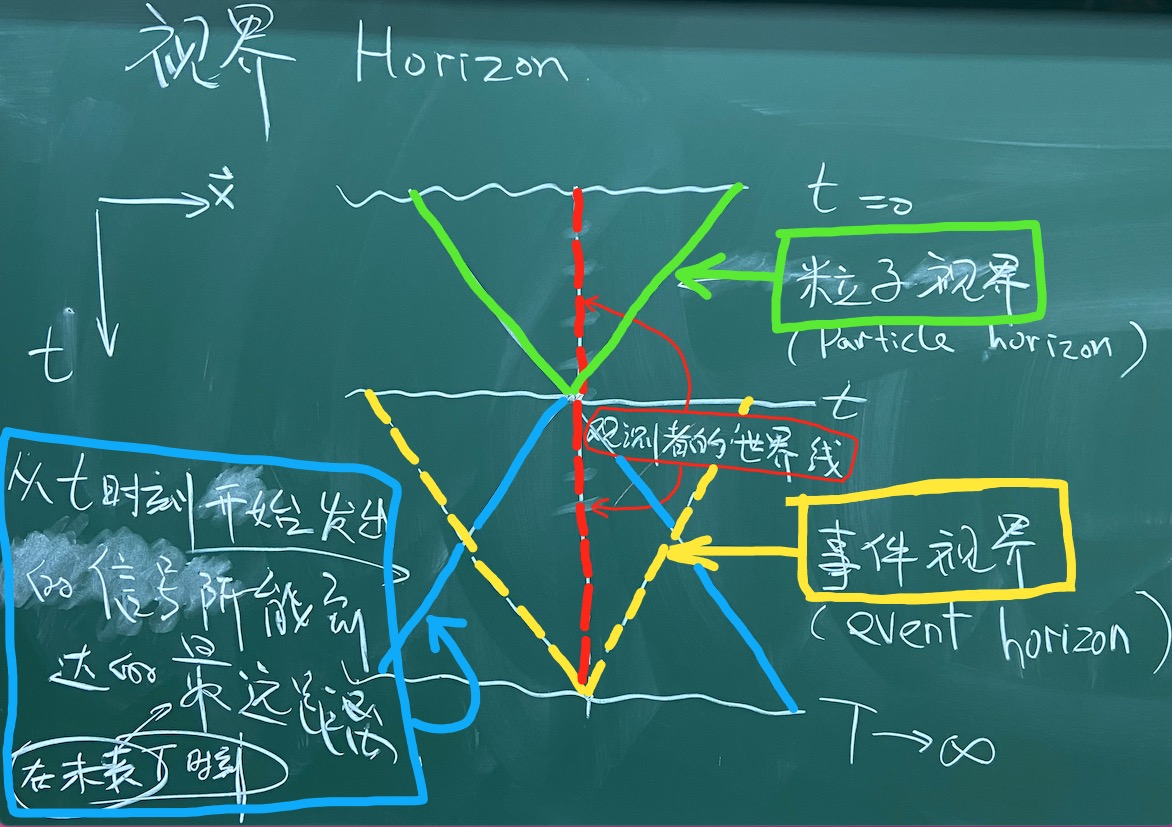
\includegraphics[width=1.0\linewidth]{horizon.jpg}
	\caption{视界}
\end{figure}

\end{document}
